

\title{Combinatorial Analysis of Semigroups, Semigroup Relations, and Semigroup Type Signatures}
\author{
        Chad Brewbaker \\
        Flying Dog Solutions\\
        13977 Summit Dr.
	Clive, Iowa 50325, \underline{U.S.A}
}
\date{\today}

\documentclass{article}
\usepackage{listings}
\lstnewenvironment{code}{\lstset{language=Haskell,basicstyle=\small}}{}
\usepackage{minted}
\usepackage{hyperref}
\usepackage{amsthm}
\usepackage{graphicx}
\graphicspath{ {img/} {znMultData/} {bmmData/}}

\newtheorem{theorem}{Theorem}[section]
\newtheorem{corollary}{Corollary}[theorem]
\newtheorem{lemma}[theorem]{Lemma}
\newtheorem{defn}[thm]{Definition}
\newtheorem{open}[thm]{Definition}
\newtheorem{exam}[thm]{Example}
\newtheorem{subroutine}[thm]{Subroutine}
%\theoremstyle{plain}
%\newtheorem{thm}{Theorem}% reset theorem numbering for each chapter

%\theoremstyle{definition}
%\newtheorem{defn}[thm]{Definition} % definition numbers are dependent on theorem numbers
%\newtheorem{exmp}[thm]{Example}



\begin{document}

\maketitle

\begin{abstract}
Semigroups are fundamental constructs in programming.   Semigroups extend groups of permutations to all bivariate functions on a finite set.   

%Open problems for semigroups include the runtime complexity of matrix-matrix multiply over a finite field [strassen, recent], primality testing [aks], and integer factorization [??]. The distributed memory parallel runtime complexity of Greatest Common Divisor is also an open problem [p complete book].  

By understanding the structure of a semigroup from first principals we are able to design precise algorithms for the semigroup. %That could be optimizing a matrix-matrix multiply, or finding a minimal sequence of machine operations on a register type.

First we inspect properties of the full transformation semigroup $T_{n}$, the semigroup of all bivariate functions over a finite set of $n$ elements.  We chase member functions under self composition (iteration) to build various directed graphs.  We then use an SMT solver [Z3] to compute minimum dominating sets. We also create directed graphs to study the interplay of semigroup multiplication between idempotent classes.

Secondly we inspect properties of permutations, boolean matrix multiplication,  modular addition, modular multiplication, and Conway's Game of Life (torus grid).  Our results include an optimal subroutine for the brute force kernel of Babai's graph isomorphism algorithm \cite{babai2015}.

Third, we extend familiar concepts like associatively and commutativity to all small relations on semigroups and enumerate their members. Results have been added to Sloane's Online Encyclopedia of Integer Sequences.

Fourth, we inspect semigroups over $n$ bit machine registers with an eye to compiler optimizations and  processor design.
%ADD, SUB,  XOR, OR, AND, NAND, SHIFTL, SHIFTR, .... Look into the machine language semigroup for an architecture.  Z_{2}, Z_{4}, Z_{8}, Z_{16}, Z_{32}, ... Which functions are not covered by iteration?
%Precicely define composition space  f:: a -> a -> a  vs bound application space g:: a -> a

% ADD :: a -> a -> a


Fifth, we demonstrate functional analogues to algebraic identities from Jr. High Algebra. It is our hope that through this lens programming can be taught alongside Algebra and reach the same level of universal education.  \end{abstract} 


%Should we do magmas too? Curious what idempotents a magma has, seems they could be completely rando.


\listoffigures


\section{Introduction}
Semigroups are sets of functions of type $f(a)\rightarrow a$ on the finite set $a$ that are closed under composition. 

In addition to mathematical notation we will also use the formal programming language Haskell \cite{hudak2007}.

\begin{code}
f :: a -> a -> a
associative f a b c  =  f( f a  b) c   ==  f a (f b c) 
\end{code}




% Alternatively, \inputminted{Haskell}{Program.hs}



Here are definitions that are used.

%Extend our results to M{n} full set of full Magmas on $n$ elements? What crazy stuff happens? All the full mult tables on $n$ elements that are not associative plus $T_{n}$.
%Magma elements still have index and period. Only our results that require associativity will break.

%Automata (rows have labels of a different type than the column labels or entries) vs binary endofunctions.

%Given a multiplication tablediscuss how to test for totality O(n^2) make sure every entry is in bounds, asssociativity, identiy O(n) look at identity row/column, divisibility, and communitivy.

\begin{defn}[Endofunction] A function with domain and co-domain of the same type.\end{defn}
\begin{defn}[Semigroup] A collection of endofunctions closed under composition.  \end{defn}
\begin{defn}[Full Transformation Semigroup on $n$ elements ] The collection of all endofunctions on an $n$ element set. Denoted $T_{n}.$\end{defn}

%\begin{exam} Multiplication table of $T_{2}$ here.\end{exam}

\begin{defn}[Iteration] Self composition of an endofunction. For $i$ self compositions on endofunction $f(x)$ we denote this as $f^{i}(x)$\end{defn}

\begin{defn}[Index] Given an endofunction, the number iterations until it enters a cycle.\end{defn}
\begin{defn}[Period] Given an endofunction, the length of the cycle under iteration.\end{defn}

\begin{defn}[Permutation] An endofunction with index of zero.\end{defn}

\begin{defn}[Symmetric group on $n$ elements] The set of all permutations on $n$ elements. Denoted $S_{n}$.\end{defn}
%\begin{exam} Multiplication table of $S_{3}$ here.\end{exam}
\begin{defn}[Idempotent] An endofunction with index of zero and period of 1.  Alternatively, $f(x) = x$ for all $x$. \end{defn}

\begin{defn}[Forgetful function] An endofunction with index of at least 1. \end{defn}
\begin{defn}[Monogenic semigroup] A semigroup generated by one element. \end{defn}

\begin{defn}[Binary Matrix Multiplication] Square matrix-matrix multiplication on the integers modulo 2. \end{defn}

%\begin{exam} Multiplication table of $BMM_{2}$ here.\end{exam}

\begin{defn}[co-BMM] Boolean matrix-matrix multiplication on the integers modulo 2 with the addition an multiplication operations swapped.\end{defn}

\begin{defn}[$Z^{+}_{n}$] Integers modulo $n$ under addition. \end{defn} 

%\begin{exam} Multiplication table of $Z^{+}_{6}$ here.\end{exam}

\begin{defn}[$Z^{\times}_{n}$] Integers modulo $n$ under multiplication. \end{defn} 

%\begin{exam} Multiplication table of $Z^{\times}_{6}$ here.\end{exam}

%\begin{tabular}{ |c |c |c |c |c |c |c | }\hline
%$Z_6^\times$&0&1&2&3&4&5\\ \hline
%0&0&0&0&0&0&0\\ \hline
%1&0&1&2&3&4&5\\ \hline
%2&0&2&4&0&2&4\\ \hline
%3&0&3&0&3&0&3\\ \hline
%4&0&4&2&0&4&2\\ \hline
%5&0&5&4&3&2&1\\ \hline
%\end{tabular}

\begin{defn}[Factoring] Given an endofunction $f$; return two endofunctions $g,h$, neither an identity function, such that $ f = g  h $.\end{defn}
\begin{defn}[Multiplication] Given endofunctions $g,h$; return an endofuction $f$, such that $ f = g h $.\end{defn}
\begin{defn}[Right division] Given endofunctions $f,h$; return an endofuction $g$, such that $ f = g h$.\end{defn}
\begin{defn}[Left division] Given endofunctions $f,g$; return an endofuction $h$, such that $ f = g h$.\end{defn}



\begin{defn}[Game of Life] Automata on orthogonal grid with binary values defined by John Conway. For this paper we will use square toroidal grids, Top/Bottom rows and Left/Right columns are considered adjacent. 
States are Live and Dead. Live cell with less than two Live neighbors dies. Live cell with 2 or 3 Live neighbors lives.  Live cell with more than 3 Live neighbors dies. Dead cell with exactly 3 live neighbors becomes Live.\end{defn} 

\begin{defn}[Detection] Given two endofunctions $f$ and $g$, if $f^{i} = g$, then $g$ is said to detect $f$. \end{defn}


%\begin{exam} Examples with permutations and $Z_{1000}^{\times}$\end{exam}


We start with a function \emph{endoscope}. It is a function on an ordered set $a$. The arguments are a list of elements in the set $a$, and an endofunction under study. It returns pairs of elements in the set under self-compositions. $(f^{0}, f^{i})$
\begin{code}
endoscope :: Ord a => [a] -> (a -> a -> a) -> Set (a,a)
\end{code}


The function \emph{idempotents} takes a list of elements and an endofunction. It returns the list of elements that are idempotent when passed through the endofunction.
\begin{code}
idempotents :: Ord a => [a] -> (a -> a -> a) -> [a]
idempotents elts mult = filter isSame elts 
       where
        isSame x = mult x x == x 
\end{code}

\begin{defin}[Leaves] Leaves are endofunctions $f$ such that for any other endofunction $g$, $f != g^{i}$ \end{defin}

\begin{defin}[Idempotent class] The idempotent class around idempotent $f f = f$ is all endofunctions $g$ such that $g^{i} = f$.    \end{defin}
The monogenic detection graph has one connected component for each idempotent class.

\begin{defin}[Cyclic member] A member with index of zero.\end{defin}

\begin{defin}[Group-likes]
Group likes are all the cyclic members of a semigroup. \end{defin}
Group-likes are similar to permutations since they have index 0.


%Crypto hash to  256 bits
%Count


%Here are the subroutines discussed.
%
%\begin{subroutine}[Boolean Matrix Multiplication] 
%
%\end{subroutine}
%
%\begin{subroutine}[Factorial] 
%
%\end{subroutine}
%
%\begin{subroutine}[Binomial Coefficent] 
%
%\end{subroutine}
%
%\begin{subroutine}[Index of endofuction] 
%
%\end{subroutine}
%
%\begin{subroutine}[Period of endofuction] 
%
%\end{subroutine}
%
%\begin{subroutine}[Primality] 
%
%\end{subroutine}
%
%\begin{subroutine}[Integer factorization] 
%
%\end{subroutine}
%
%\begin{subroutine}[Integer addition] 
%
%\end{subroutine}
%
%\begin{subroutine}[Integer multiplication]

%Grid method: $O({log(n)^2 \over p})$ O(1) multiplications for each digit pair followed by a reduction of their products.

%F{\"u}rer's method \cite{furer2007} approaches a conjectured lower bound of $O(n log n)$.
%\end{subroutine}

\section{The Full Transformation Semigroup, $T_{n}$}
The as an analogue to Cayley's Theorem for groups of permutations, all sets of endofunctions form a subsemigroup of the full transformation semigroup $T_{n}$.  By making designing our analysis techniques to work on any subseimgroup of $T_{n}$ we design analysis techniques that work on every semigroup.

\subsection{Edges under iteration}
We denote an edge if $f^i(x) = g(x)$.

\inputminted{text}{tnEdges.seq}

\subsection{Idempotents (connected components)}
\inputminted{text}{tnIdempotents.seq}
\subsection{Histogram of index,period.}

\subsection{Forgetful functions} Recall, endofunctions which are not permutations were called ``reluctant" \cite{mullin1970}. Under self composition they form tree like structures which under self composition forget states in their co-domain until they reach a cycle with no further loss of co-domain elements.

\subsection{Leaves}
\inputminted{text}{tnLeaves.seq}
\subsection{Group-likes}
Group likes are all the cyclic members of a semigroup. They behave like permutations since they have index 0.

% f^i =  f,g,h,f  -> [(f,g), (g,h), (h,f)]
\subsection{Monogenic Transition Graph}
This is the graph of individual edges induced by the set of functions under iteration.

\subsection{Monogenic Reachability Graph}
This is the Monogenic Transition Graph where edges under transitive closure are also added. i.e. if $f^{i}=g$ then we place an edge $f \rightarrow g$.

\subsection{Monogenic Detection Graph}
This is the dual of the Monogenic Reachabiliy graph. Edges are reversed in direction, and loops are added to. We call this the "detection" graph because if $f^{i}=g$ then it can be said that the existence of the function $g$ must hold when $f$ exists, so $g$ can be used as a proxy to test the non-existance of $f$.


\subsection{Min Dom Set}
Using the Microsoft Z3 SMT solver we compute minimum dominating sets of our monogenic graphs.





\subsection{Idempotent mult table}
What happens if we rewrite a the mutliplication table $ [(a,b,c)]$ with [id(a),id(b),id(c) ]? 


\subsection{composition complexity}
Some functions take larger resources than others to execute. We can use dynamic programming to derive a composition chain that is minimal. For instance in elementary school we learned that multiplying by 10 simply added a zero, which can be less complex than multiplying by other numbers.

\begin{code}
[(complexity, (a -> a))]
\end{code}

In the case of matrix matrix multiply, the complexity might be $N$ times the number of nonzero elements in the right hand matrix.


\subsection{Homogenious idempontent products}

Given two elements having the same idempotent under self composition, how can we effectively efficently multiply them?


\subsection{Equivalence classes of multiplications by idempotent}
Let $idemp(a)$ be the function that maps $a$ to it's idempotent under self iteration.
Let $a\times b = c$, be denoted as $(a,b,c)$. We map $(a,b,c)$ to $(idemp(a), idemp(b), idemp(c)$ to form multiplication equivalence classes over idempotents. 

The number of idempotent equivalent multiplications for the full transformation semigroup $T_{n}$ is: 1, 11, 268, 13705.  (TODO SUBMIT TO OEIS) 

Hopefully we can use these equivalence classes to compress the information/work needed to perform arbitrary multiplications for the endofunction.

For $Z_{n}$ under multiplication the sequence seems to be $4^{prime divisors}$.


\section{Permutation function spaces, $S_{n}$}



\begin{code}
perm :: a -> a
-- perm must be a cycle under iteration 
\end{code}


Edges under iteration

Idempotents (connected components)

Histogram of index,period.

Reluctant functions: By definition permutation function sets have no reluctant functions.

Leaves

Group-likes

\subsection{Min Dom Set}
The size of a min dominating set for the monogenic inclusion graph of $S_{n}$ is \href{https://oeis.org/A186202}{OEIS A186202}. 

$$\sum_{p}^{n} \sum_{i=1}^{\lfloor {n\over p}\rfloor} {n! \over (n-ip)!i!p^{i}(p-1)   }$$


The sequence starting at $n=0$ is: 0, 1, 4, 13, 41, 151, 652, 2675, 10579, 59071, 711536, 6180307, 76629775, 873676259, 7496233396, 49493077951.

Publication of this result was declined by TCS \cite{babai2008}, with the irony that it would be come an optimal subroutine seven years later in \cite{babai2015} to replace the ``brute force enumeration" of the symmetric group.


\section{Multiplication in $Z_{n}$ }

Edges under iteration

Edges in monogenic inclusion graph of $Z_n^{*}$:
\inputminted{text}{monoZnEdges.seq}

\begin{figure}[h]
\centering
\caption{$Z_{6}^{*}$ Mono Transition Graph}
\includegraphics[width=0.5\textwidth]{z6MT.png}
\end{figure}

\begin{figure}[h]
\centering
\caption{$Z_{7}^{*}$ Mono Transition Graph}
\includegraphics[width=0.5\textwidth]{z7MT.png}
\end{figure}


\begin{figure}[h]
\centering
\caption{$Z_{6}^{*}$ Min Dom Set on Mono Transition Graph}
\includegraphics[width=0.5\textwidth]{z6MT_min_dom.png}
\end{figure}

\begin{figure}[h]
\centering
\caption{$Z_{7}^{*}$ Min Dom Set on Mono Transition Graph}
\includegraphics[width=0.5\textwidth]{z7MT_min_dom.png}
\end{figure}

\begin{figure}[h]
\centering
\caption{$Z_{6}^{*}$ Mono Detection Graph}
\includegraphics[width=0.5\textwidth]{z6MD.png}
\end{figure}

\begin{figure}[h]
\centering
\caption{$Z_{7}^{*}$ Mono Detection Graph}
\includegraphics[width=0.5\textwidth]{z7MD.png}
\end{figure}


\begin{figure}[h]
\centering
\caption{$Z_{6}^{*}$ Min Dom Set on Mono Detection Graph}
\includegraphics[width=0.5\textwidth]{z6MD_min_dom.png}
\end{figure}


\begin{figure}[h]
\centering
\caption{$Z_{7}^{*}$ Min Dom Set on Mono Detection Graph}
\includegraphics[width=0.5\textwidth]{z7MD_min_dom.png}
\end{figure}

\begin{figure}[h]
\centering
\caption{$Z_{6}^{*}$ Mono Reachability Graph}
\includegraphics[width=0.5\textwidth]{z6MR.png}
\end{figure}

\begin{figure}[h]
\centering
\caption{$Z_{7}^{*}$ Mono Reachability Graph}
\includegraphics[width=0.5\textwidth]{z7MR.png}
\end{figure}


\begin{figure}[h]
\centering
\caption{$Z_{6}^{*}$ Min Dom Set on Mono Reachability Graph}
\includegraphics[width=0.5\textwidth]{z6MR_min_dom.png}
\end{figure}

\begin{figure}[h]
\centering
\caption{$Z_{7}^{*}$ Min Dom Set on Mono Reachability Graph}
\includegraphics[width=0.5\textwidth]{z7MR_min_dom.png}
\end{figure}



%\includegraphics[height=5cm]{znMultData/z7MT.png}
\newpage
Idempotents (connected components)

Histogram of index,period.

Reluctant functions

Leaves

Group-likes

What does this tell us about integer factorization?


\section{Addition in $Z_{n}$ }

Edges under iteration
\href{http://www.oeis.org/A057660}{OEIS A057660}, the sum of orders of elements in a cyclic group with $n$ elements. $$\sum_{k=1..n} {n \over GCD(n,k)}$$

Idempotents (connected components)

Histogram of index,period.

Reluctant functions

Leaves

Group-likes



\section{Boolean matrix multiplication }
Boolean ($Z_{2}$) matrix-matrix multiplication (BMM) is a fundamental subroutine. Computations from transitive closure to parsing context free grammars\cite{valiant1975} reduce to BMM.

Traditionally the complexity of BMM is written by $O(n^{\omega})$, where $\omega$ shrinks from the brute force value of $3$ as researchers since Strassen have derived more efficient BMM algorithms.

Endoscope groups matrices into connected components under self composition. 
%My personal conjecture is that BMM is $O((n log n)^{2} )$ (Chad)
% http://math.stanford.edu/~church/BCCGU-On-cap-sets-and-the-group-theoretic-approach-to-matrix-multiplication.pdf Note that the Umans conjecture for \omega=2 was just disproven.
% bmm :: m -> m -> m
% $m^{m \times m}$ is the function space where $m$ is a set the size $2^{m \times m}$
%Of course we aren't grabbing all functions from that pair, just those that are legal BMM results.
%Can we come up with a compression method formulation as a BMM lower bound?
%Compress the serialized m,m,m triples into FSA. Do FSA minimization. Feasible on 3x3 BMM? (2^{9})*(2^{9}) words in the language. All words length 27.
%What permutation of these triples allows us to reduce average rejection prefix for an illegal word? Thats feasible for 2x2 BMM very quickly.

Edges under iteration

Idempotents (connected components), same as fixed points?

Histogram of index,period.

Forgetfull functions

Leaves

Group-likes

\subsection{Min dom set}
The minimum dominating set for 1x1 matrices over $Z_{n}$ is https://oeis.org/A034444, the number of squarefree divisors.
The minimum dominating set for 2x2 matrices over $Z_{n}$ is https://oeis.org/A226756.

%Do we even need to shell out to Z3? The min dom set is just the idempotents? Is this a bug because we need to remove the idempotents first?





What does this tell us about the complexity of BMM?


\begin{figure}[h]
\centering
\caption{$BMM_{2}$ Min Dom Set }
\includegraphics[width=0.5\textwidth]{"bmmData/2MD_min_dom"}
\end{figure}

Note: Igro Potapov has some results on ZNMM %, https://scholar.google.com/citations?view_op=view_citation&hl=en&user=zdGjSYAAAAAJ&sortby=pubdate&citation_for_view=zdGjSYAAAAAJ:W5xh706n7nkC

\subsection{Complexity of Strassen style matmul}
Strassen style matrix multiplications rely on an interleaving of sparse multiplies and additions of matrices over $Z_{k}(n,n)$


1) Endofuction of matrix multiply over  $Z_{k}(n,n)$.
2) Endofuction of matrix add over  $Z_{k}(n,n)$.

Elements now have two outputs upon iteration. What do these graphs look like? What is their min detection set if we ignoring idempotents?

DAG of add or multily. Can use source or a constant



\subsection{Brent equations}
$\delta_{i,j}$, the Kronecker delta function, is 0 if $i \neq j$ and 1 if $i =j$.

$\sum_{i=1}^{r} A_{ij}^(i) B_{kl}^{i} C_{mn}^{i} = \delta_{n,i}\delta_{j,k}\delta_{l,m}$






\section{Boolean matrix co-multiplication }
We define boolean matrix-matrix co-multiply (co-BMM) as the function where we have swapped the multiply and addition operators. 

As a data type, each resulting entry is the $n$-tuple consisting of entries that are either $A_{i,k}$ or $B_{k,j}$. If view $A$ and $B$ as graphs, with rows being outgoing edges and columns as incoming edges; we have $n$-tuples of chosing either the incoming or outgoing edge for each entry.


Edges under iteration

Idempotents (connected components), same as fixed points?

Histogram of index,period.

Forgetful functions

Leaves

Group-likes


What does this tell us about the complexity of co-BMM?

\section{Transformation polynomials }
In \cite{ashlock1990} the concept of a permutation polynomial over $Z_{n}$ was studied. These are polynomials with coefficients and powers from $Z_{n}$ that form a permutation function on $Z_{n}$. We extend this concept to all polynomials with coefficients and powers from $Z_{n}$. 

Note that when $n$ is prime then all $n^n$ transformations exist, but when $n$ is a composite such as 4 or 6, then the distinct transformations is exponentially smaller. Here are the values for small $n$ starting at $n=1$.
\inputminted{text}{transpoly.seq}

Interestingly, this would seem to imply that transformation polynomials form a generalization of the AKS\cite{agrawal2004} class of primality tests. We can enumerate the polynomials over $Z_{n}$, claiming ``composite" when two polynomials make an equivalent transformation, and ``prime" when we have shown all are unique or all are unique up to some AKS style bound. 


\subsection{Functions in set}
In \cite{bhargava2000} the formula for the number of polynomial functions in $Z_{n}$ was derived to be, $$\prod_{k=0}^{n-1} {n\over gcd(n, k!)} $$.

Edges under iteration

Idempotents (connected components), same as fixed points?

Histogram of index,period.

Reluctant functions

Leaves

Group-likes


What does this tell us about the complexity of primality testsing and factoring?


\section{Compositional equality relations}

\section{Applications}
Alon \cite{alon1985} demonstrated an application of endofuction composition for optimizing network transfers.

\section{Scratch}
Scratch space for musings. 
\subsection{AKS Primality endofuction}
%In \cite{anderson2005}  proved that an iterated endofuction 

Borwein \cite{borwein1985} showed us that computing $n!$ by successive multiplications was rather inneficient.

$$8! =2*3*2^{2}*5*(2*3)*7*(2^{3})$$

Instead, we can take the table of all primes up to $n$, figure out how many times each prime factor is applied and exponentiate each prime factor once to the appropriate power.
$$8! = 2^{7}*3^{2}*5*7$$

Geotgheluck showed us how to compute binomial coefficients using prime factorizations, \cite{goetgheluck1987, goetgheluck1988}.


% Chad 
%Is Geotgheluck's method any faster than applying Borwein's to $n!, k!, (n-k)! $ then subtracting the denominator exponents?

AKS\cite{agrawal2004} noted that for prime numbers ${n \choose k}$ always is divisible by  $n$, since no term in the denominator less than $n$ is a factor. ${n! \over k! * (n-k)!}$

However for composite numbers $n$ , some values of ${n \choose k}$ are not divisible by $n$.

\begin{code}
aksBinomial :: Integer -> Integer -> Integer
aksBinomial n k = mod (binomial n k) n
\end{code}

When this function returns a nonzero value, we know that $n$ is a composite number.

% $p(x)\equiv q(x)$ mod $(x^{r}-1 ,n)$ denotes both $p(x)\equiv q(x)$ mod $x^{r}-1$ and $p(x)\equiv q(x)$ mod $n$.

% Chad
% Can we use Borwein factorial simplification to cheat? Know that if $n$ is not prime then we don't need another entry into our prime table. $n$ will be a composite of others. With k= n-1 
% binomial n k = binomial (n-1) (k-1) +  binomial (n-1) k

%\prod_{i=1}^{k} {n +1 + i) \over i } \prod_{i=1}^{k} {n -(k -i)) \over i }


% If $k$ is  sqrt(n) +1 then either that bottom $k!$ whacks out a chuck, or it leaves that largest number unfactored.
%can we take successive $2^{i}!$ to find the order of magnitude of the smallest prime divisor?


Enumerating trees of binary and unary functions:

Sets of binary/unary function equaltities

\section{Semigroup Type Signatures}


\begin{theorem}[Exponentials]
The number of functions from a size $y$ set to a size $x$ set is }$x^{y}$. 
\end{theorem}

This relation between exponentials and functions gives a translation between algebraic and functional viewpoints.

%It is no coincidence that John Atanasoff, inventor of the first electronic digital computer, had an early curiosity with exponents and logarithms \cite{boyanov2003}.

Magmas are two variable functions with type signature:
\begin{code}
magma :: a -> a -> a
\end{code}

\begin{corollary}
The order of an unconstrained magma is $n^{n^{n}}$.
\end{corollary}

The complete semigroup on $n$ elements is called the full transformation semigroup denoted as $T_{n}$

\begin{corollary}
The full transformation semigroup has order $n^{n}$.
\end{corollary}

Recall this algebraic identity:

$$(a^{m})^{n} = a^{mn}$$

Translated from exponential notation into functional notation we have:
\begin{code}
curry :: n -> m -> a
curry' :: (n,m) -> a
\end{code}
We name these functions ``curry" in reference to Haskell Curry \cite{curry1934}. Curry's rule states we can refactor between a function between passing multiple arguments, a function that passes a tuple of values, and chaining of functions.

For functions with two arguments $f(a,a)\rightarrow a$, Author Cayley \cite{cayley1851} noted we can abstract them into multiplication tables. Applying Curry's rule we can bind the first argument in the multiplication resulting in a function with one argument. All three of these type signatures are of the same order:
\begin{code}
f :: (a,a) -> a
g :: a -> a -> a
h :: a -> (a -> a)
\end{code}

% I can never remember how to format umlauts etc in latex, http://tex.stackexchange.com/questions/57743/how-to-write-�-and-other-umlauts-and-accented-letters-in-bibliography (Chad)

J. Richard B\"{u}chi \cite{buchi1962} further described how we can use either multiplication tables, transition graphs, or transition trees to give us a viewpoint that best fits a discussion on magmas. A quality English translation was made by Sylvia B\"{u}chi, Peter Deussen and Dirk Siefkes \cite{maclane1990}.

\begin{figure}[h]
    \centering
    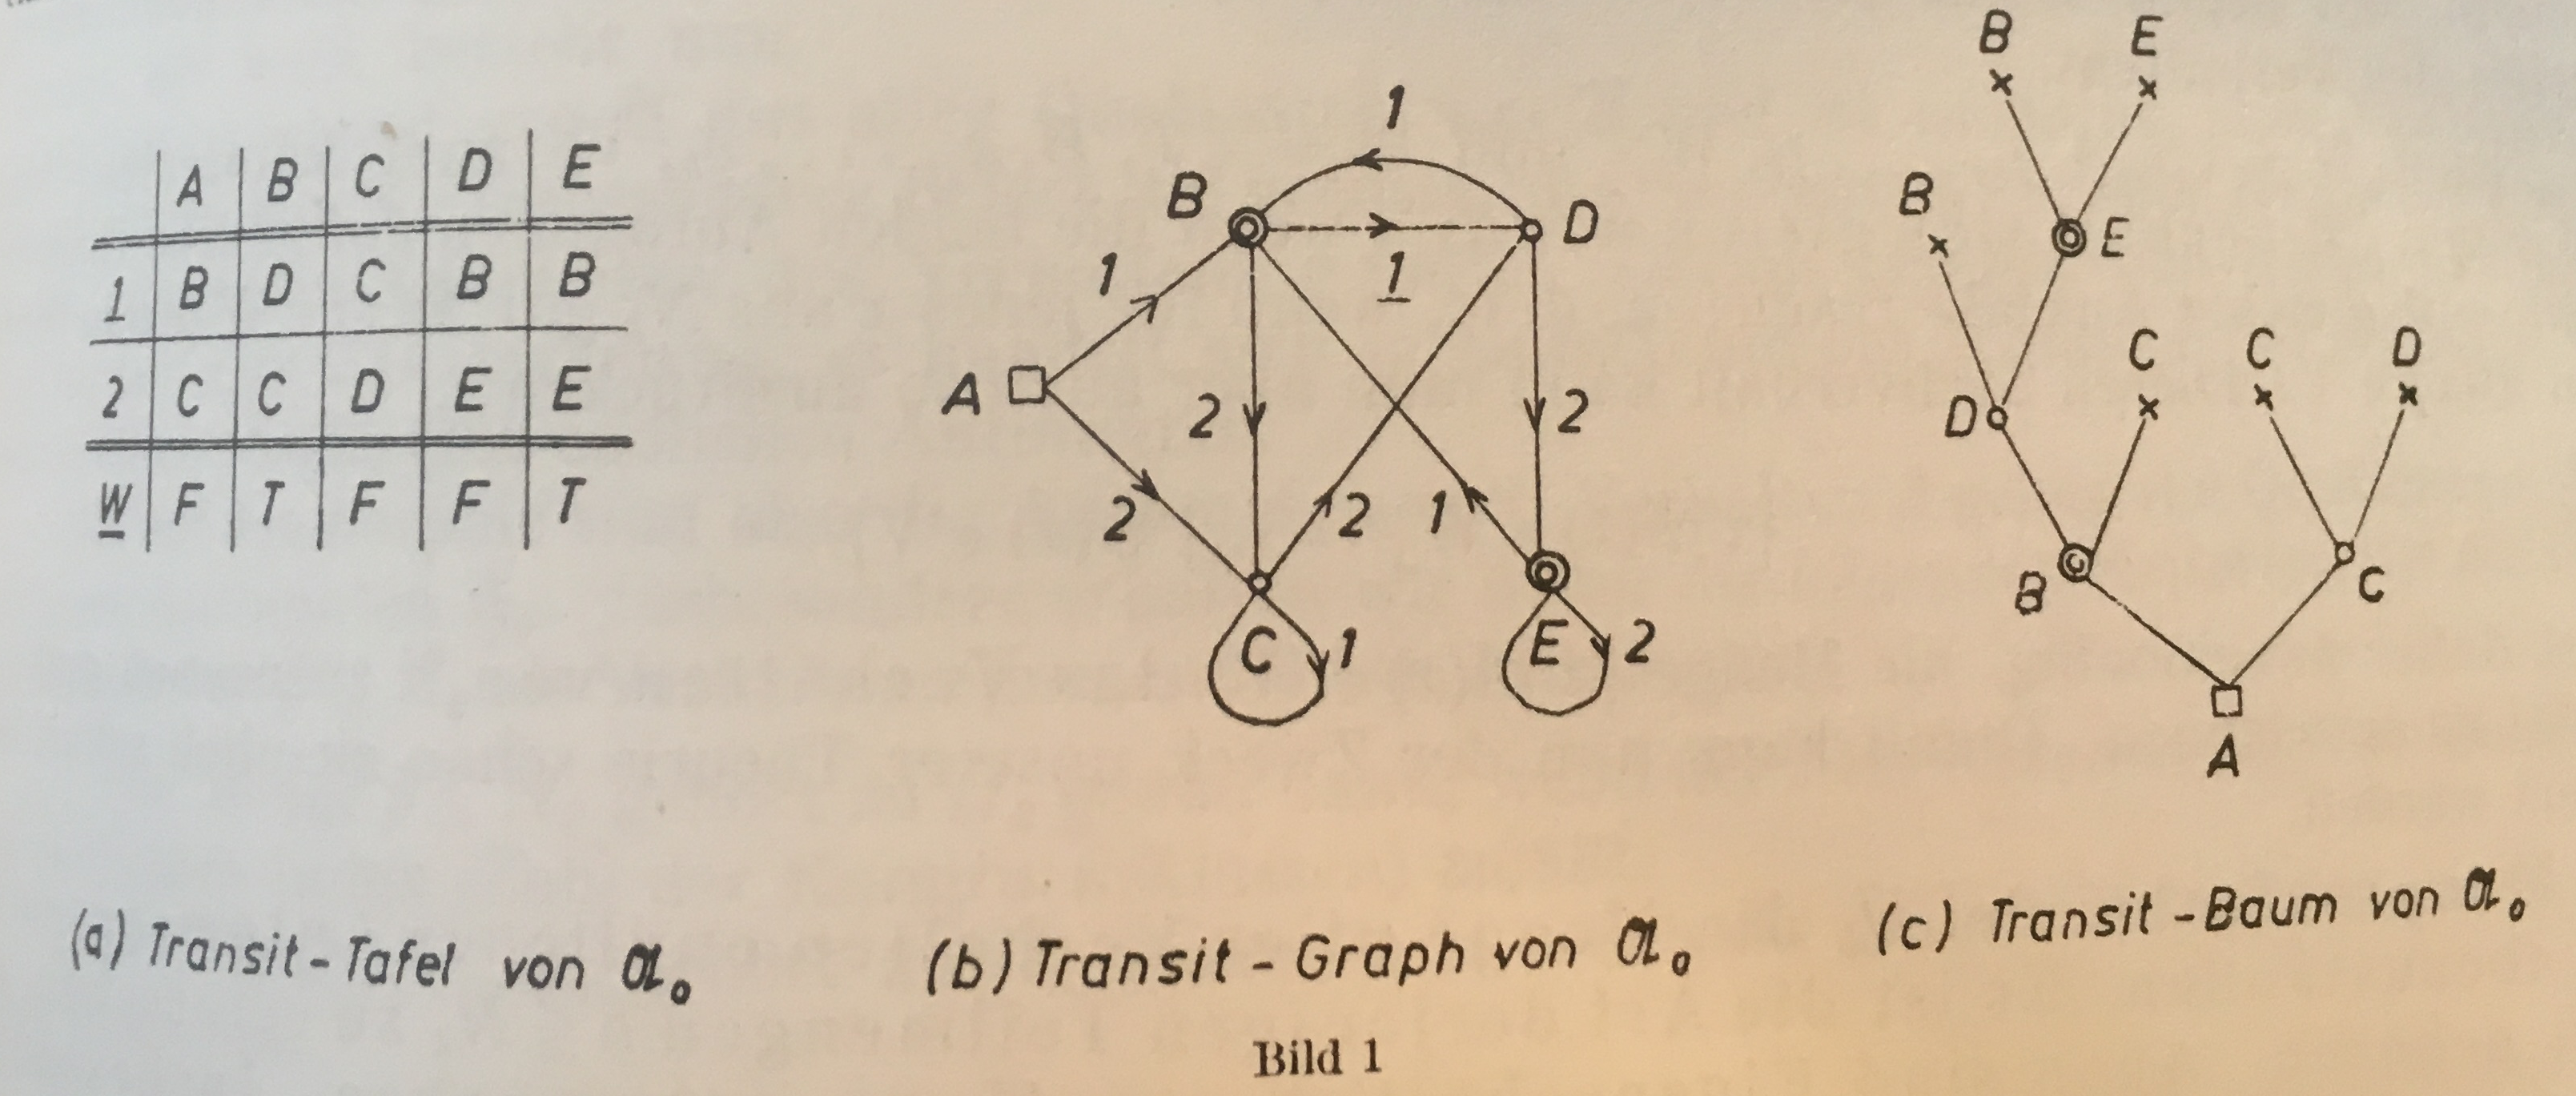
\includegraphics[height=4cm]{buchiTrinity}
    \caption{Diagram made by B\"{u}chi}
   
\end{figure}


Multiplication table function
\begin{code}
multTableFunc :: a -> a ->a
\end{code} 

Binding the first variable on all possible values gives a list of functions:
\begin{code}
boundList ::  [(a->a)]
\end{code}

The enumeration of all triples is the multiplication table:
\begin{code}
 multTable :: [(a,a,a)]
\end{code}



\section{Conclusion and open problems}
\begin{open}[Boolean Matrix Matrix Mulitiply] What is the runtime complexity of Boolean matrix-matrix multiply?\end{open}

What is the runtime complexity of integer factorization?

What is the runtime complexity of primality testing?

What is the distributed memory parallel complexity of greatest common divisor?

How many semigroup type signatures are there in the LLVM compiler suite? (Or an entire Linux distribution)  How many functions do they correspond to and which are the fastest?

Study the semigroup of common assembly language functions like OR, AND, XOR, ADD , SUB, NOT, MULT over $Z_{2^{k}}$.  What does it tell us about compiler optimizations or machine instructions that would be useful?


\appendix{New OEIS Sequences}

\appendix{Haskell source}

\nocite{*}
\bibliographystyle{plain}
\bibliography{biblio}
\end{document}
